\documentclass{article}

% Language setting
% Replace `english' with e.g. `spanish' to change the document language
\usepackage[english]{babel}

% Set page size and margins
% Replace `letterpaper' with `a4paper' for UK/EU standard size
\usepackage[letterpaper,top=2cm,bottom=2cm,left=3cm,right=3cm,marginparwidth=1.75cm]{geometry}

% Useful packages
\usepackage{amsmath}
\usepackage{graphicx}
\usepackage{mathbbol}
\usepackage{amsthm}
\usepackage{amssymb}
\usepackage[colorlinks=true, allcolors=blue]{hyperref}

% Font size
\usepackage{setspace}
\doublespacing

% tree
\usepackage{tikz}

\title{CSCB63 Assignment 1}
\author{Zheyuan Wei}

\begin{document}
\maketitle

\section*{Q1}

\subsection*{Q1-a}


\text{Q: }
$ If\ f(n) \in \mathcal{O}(g)\ and\ g \in \mathcal{O}(h)\ then\ f \in \mathcal{O}(h), for\ all\ f, g, h \ in\ \mathbb{N} \rightarrow \mathbb{R^+} $

\begin{proof}

    \text{\newline}

    $ \text{1) From } f \in \text{O(g)} \ we\ have: $
    $$ \exists c_1, n_1 \in \mathbb{R} \text{ s.t. } f(n) \leq c_1 \cdot g(n) \forall n \geq n_1 $$

    $ \text{2) From } g \in \text{O(h)} \ we\ have: $
    $$ \exists c_2, n_2 \in \mathbb{R} \text{ s.t. } g(n) \leq c_2 \cdot h(n) \forall n \geq n_2 $$

    $ \text{3) From 1) \ and\ 2) \ we\ have: }$
    $$ f(x)=\left\{
        \begin{aligned}
            f(n) \leq c_1 \cdot g(n) \forall n \geq n_0, & \text{for some $c_1$ and $n_1$} \\
            g(n) \leq c_2 \cdot h(n) \forall n \geq n_1, & \text{for some $c_2$ and $n_2$} \\
        \end{aligned}
        \right.\\
        \Rightarrow
        \begin{aligned}
            f(n) \leq c_1 ( c_2 \cdot h(n) ) \forall s.t.
            \left\{
            \begin{aligned}
                n \geq n_1 \\
                n \geq n_2 \\
            \end{aligned}
            \right.
        \end{aligned}
    $$
    $ \text{4) From 3) \ we\ have: }$
    $$ f(n) \leq c_1 \cdot c_2 \cdot h(n)\ \forall n \geq max(n_1, n_2) $$
    $$ \Rightarrow f \in \mathcal{O}(h) $$
    % $$ \blacksquare $$

\end{proof}

\newpage

\subsection*{Q1-b}

\text{Q: }
$ If\ f \in \Omega(g)\ and\ g \in \Omega(h)\ then\ f \in \Omega(h), for\ all\ f, g, h\ in\ \mathbb{N} \rightarrow \mathbb{R^+} $

\begin{proof}

    \text{\newline}

    $ \text{1) From} \ f \in \Omega(g) \ \text{we have: } $
    $$ \exists c_1, n_1 \in \mathbb{R} \text{ s.t. } f(n) \geq c_1 \cdot g(n) \forall n \geq n_1 $$

    $ \text{2) From} \ g \in \Omega(h) \ \text{we have: } $
    $$ \exists c_2, n_2 \in \mathbb{R} \text{ s.t. } g(n) \geq c_2 \cdot h(n) \forall n \geq n_2 $$

    $ \text{3) From 1) \ and\ 2) \ we\ have: }$
    $$ f(x)=\left\{
        \begin{aligned}
            f(n) \geq c_1 \cdot g(n) \forall n \geq n_0, & \text{for some $c_1$ and $n_1$} \\
            g(n) \geq c_2 \cdot h(n) \forall n \geq n_1, & \text{for some $c_2$ and $n_2$} \\
        \end{aligned}
        \right.\\
        \Rightarrow
        \begin{aligned}
            f(n) \geq c_1 ( c_2 \cdot h(n) ) \forall s.t.
            \left\{
            \begin{aligned}
                n \geq n_0 \\
                n \geq n_1 \\
            \end{aligned}
            \right.
        \end{aligned}
    $$

    $ \text{4) From 3) \ we\ have: }$
    $$ f(n) \geq c_1 \cdot c_2 \cdot h(n)\ \forall n \geq max(n_0, n_1) $$
    $$ \Rightarrow f \in \Omega(h) $$
    % $$ \blacksquare $$

\end{proof}

\newpage

\subsection*{Q1-c}
\text{Q: \\}
$ \log_\phi(\sqrt{5}(n+2)) - 2 \in \mathcal{O}(\log_2(n)) $
$ \text{where} \ \phi \text{ is the golden ratio.} $

\begin{proof}

    $ \text{Let } f(n) = \log_\phi(\sqrt{5}(n+2)) - 2, \forall n \geq 0 $

    $ \text{Then it follows that: } $

    $$ f(n) = \log_\phi(\sqrt{5}(n+2)) - 2 = \frac{\log_2(\sqrt{5}(n+2))}{\log_2(\phi)} - 2 $$
    $$ f(n) = \frac{\log_\phi{\sqrt{5}}}{\log_2(\phi)} \cdot \log_2(n+2) - 2 $$
    $$ f(n) < \frac{\log_\phi{\sqrt{5}}}{\log_2(\phi)} \cdot \log_2(n+2) = k \cdot \log_2(n+2) \ \forall n \geq 0 $$
    $ \text{where } k = \frac{\log_\phi{\sqrt{5}}}{\log_2(\phi)} \in \mathbb{R} $
    $$ \Rightarrow f(n) < k \cdot \log_2(n+2) \leq k \cdot \log_2(n^2) = k \cdot 2 \cdot \log_2(n) \ \forall n \geq 2 $$
    $ \text{which is equivalent to: } $
    $$ f(n) < 2k \cdot \log_2(n) \ \forall n \geq 2 $$
    $$ \Rightarrow f(n) \in \mathcal{O}(\log_2(n)) $$
    % $$ \blacksquare $$
\end{proof}

\newpage

\section*{Q2}

\subsection*{Q2-a}

\text{Q: }
\text{On an initially empty tree, show each step of inserting the keys 9, 10, 12, 14, 3, 34, 19, 37, 20. }

\paragraph{Step 1: Insert 9 \\}
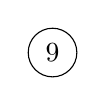
\begin{tikzpicture}[every node/.style={draw,circle,minimum size=3ex}]
    \node (root) {9};
\end{tikzpicture}

\paragraph{Step 2: Insert 10 \\}
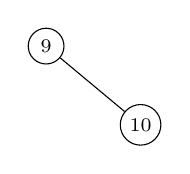
\begin{tikzpicture}[%level distance=5mm,
        level 1/.style={level distance=10mm,sibling distance=24mm},
        level 2/.style={level distance=10mm,sibling distance=16mm},
        level 3/.style={level distance=8mm,sibling distance=8mm},
        font=\scriptsize,inner sep=2pt,every node/.style={draw,circle,minimum size=3ex}]

    \node {9}
    child [missing]
    child   {node {10}}; % right child
\end{tikzpicture}

\paragraph{Step 3: Insert 12 \\}
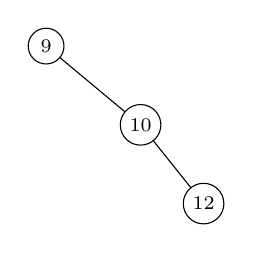
\begin{tikzpicture}[%level distance=5mm,
        level 1/.style={level distance=10mm,sibling distance=24mm},
        level 2/.style={level distance=10mm,sibling distance=16mm},
        level 3/.style={level distance=8mm,sibling distance=8mm},
        font=\scriptsize,inner sep=2pt,every node/.style={draw,circle,minimum size=3ex}]

    \node {9}
    child [missing] % left child
    child   {node {10} % right child
            child [missing] % level 2
            child   {node {12}}};
\end{tikzpicture}
\\
Imbalanced. Right heavy. \\
Need a left rotation. \\
Left rotation: \\\\
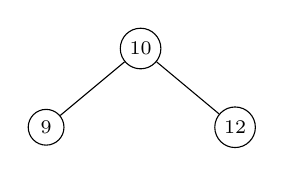
\begin{tikzpicture}[%level distance=5mm,
        level 1/.style={level distance=10mm,sibling distance=24mm},
        level 2/.style={level distance=10mm,sibling distance=16mm},
        level 3/.style={level distance=8mm,sibling distance=8mm},
        font=\scriptsize,inner sep=2pt,every node/.style={draw,circle,minimum size=3ex}]

    \node {10}
    child   {node {9}}
    child   {node {12}};
\end{tikzpicture}

\paragraph{Step 4: Insert 14 \\}
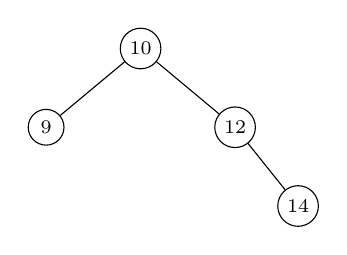
\begin{tikzpicture}[%level distance=5mm,
        level 1/.style={level distance=10mm,sibling distance=24mm},
        level 2/.style={level distance=10mm,sibling distance=16mm},
        level 3/.style={level distance=8mm,sibling distance=8mm},
        font=\scriptsize,inner sep=2pt,every node/.style={draw,circle,minimum size=3ex}]

    \node {10}
    child   {node {9}}
    child   {node {12}
            child [missing]
            child   {node {14}}};
\end{tikzpicture}

\paragraph{Step 5: Insert 3 \\}
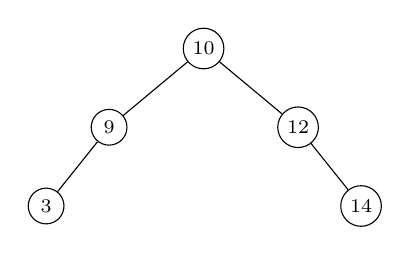
\begin{tikzpicture}[%level distance=5mm,
        level 1/.style={level distance=10mm,sibling distance=24mm},
        level 2/.style={level distance=10mm,sibling distance=16mm},
        level 3/.style={level distance=8mm,sibling distance=8mm},
        font=\scriptsize,inner sep=2pt,every node/.style={draw,circle,minimum size=3ex}]

    \node {10}
    child   {node {9}
            child   {node {3}}
            child [missing]}
    child   {node {12}
            child [missing]
            child   {node {14}}};
\end{tikzpicture}

\paragraph{Step 6: Insert 34 \\}
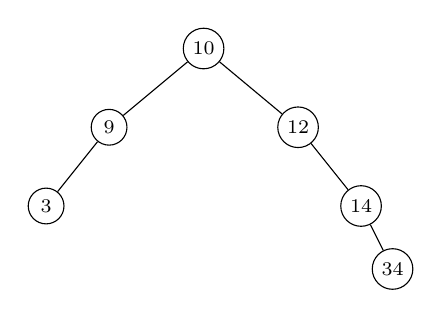
\begin{tikzpicture}[%level distance=5mm,
        level 1/.style={level distance=10mm,sibling distance=24mm},
        level 2/.style={level distance=10mm,sibling distance=16mm},
        level 3/.style={level distance=8mm,sibling distance=8mm},
        level 4/.style={level distance=8mm,sibling distance=4mm},
        font=\scriptsize,inner sep=2pt,every node/.style={draw,circle,minimum size=3ex}]

    \node {10}
    child   {node {9}
            child   {node {3}}
            child [missing]}
    child   {node {12}
            child [missing]
            child   {node {14}
                    child [missing]
                    child   {node {34}}}};
\end{tikzpicture}
\\
Imbalanced. Right heavy. \\
Need a left rotation. \\
Left rotation: \\\\
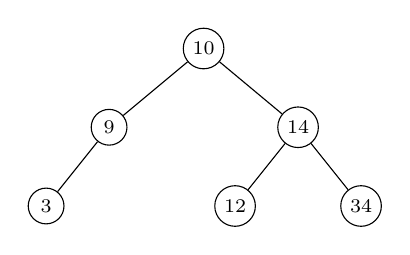
\begin{tikzpicture}[%level distance=5mm,
        level 1/.style={level distance=10mm,sibling distance=24mm},
        level 2/.style={level distance=10mm,sibling distance=16mm},
        level 3/.style={level distance=8mm,sibling distance=8mm},
        font=\scriptsize,inner sep=2pt,every node/.style={draw,circle,minimum size=3ex}]

    \node {10}
    child   {node {9}
            child   {node {3}}
            child [missing]}
    child   {node {14}
            child   {node {12}}
            child   {node {34}}};
\end{tikzpicture}

\paragraph{Step 7: Insert 19 \\}
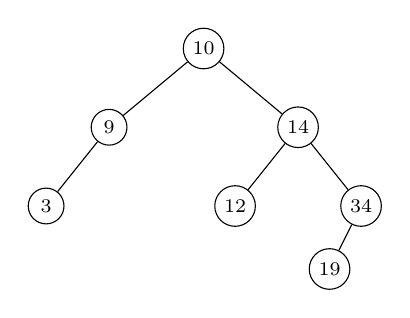
\begin{tikzpicture}[%level distance=5mm,
        level 1/.style={level distance=10mm,sibling distance=24mm},
        level 2/.style={level distance=10mm,sibling distance=16mm},
        level 3/.style={level distance=8mm,sibling distance=8mm},
        level 4/.style={level distance=8mm,sibling distance=4mm},
        font=\scriptsize,inner sep=2pt,every node/.style={draw,circle,minimum size=3ex}]

    \node {10}
    child   {node {9}
            child   {node {3}}
            child [missing]}
    child   {node {14}
            child   {node {12}}
            child   {node {34}
                    child   {node {19}}
                    child [missing]}};
\end{tikzpicture}

\paragraph{Step 8: Insert 37 \\}
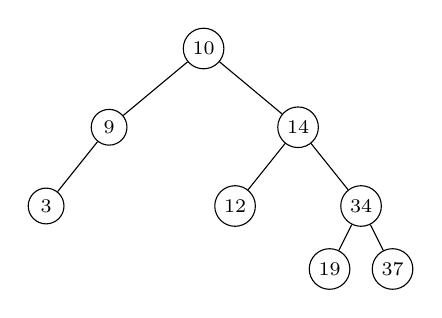
\begin{tikzpicture}[%level distance=5mm,
        level 1/.style={level distance=10mm,sibling distance=24mm},
        level 2/.style={level distance=10mm,sibling distance=16mm},
        level 3/.style={level distance=8mm,sibling distance=8mm},
        level 4/.style={level distance=8mm,sibling distance=4mm},
        font=\scriptsize,inner sep=2pt,every node/.style={draw,circle,minimum size=3ex}]

    \node {10}
    child   {node {9}
            child   {node {3}}
            child [missing]}
    child   {node {14}
            child   {node {12}}
            child   {node {34}
                    child   {node {19}}
                    child   {node {37}}}};
\end{tikzpicture}

\paragraph{Step 9: Insert 20 \\}
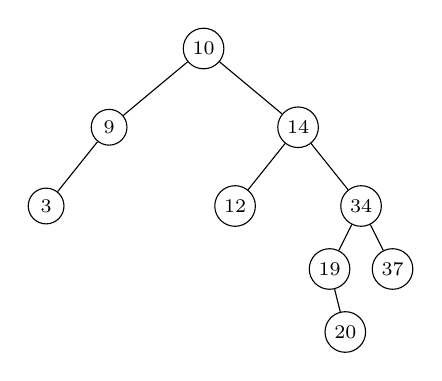
\begin{tikzpicture}[%level distance=5mm,
        level 1/.style={level distance=10mm,sibling distance=24mm},
        level 2/.style={level distance=10mm,sibling distance=16mm},
        level 3/.style={level distance=8mm,sibling distance=8mm},
        level 4/.style={level distance=8mm,sibling distance=4mm},
        font=\scriptsize,inner sep=2pt,every node/.style={draw,circle,minimum size=3ex}]

    \node {10}
    child   {node {9}
            child   {node {3}}
            child [missing]}
    child   {node {14}
            child   {node {12}}
            child   {node {34}
                    child   {node {19}
                            child [missing]
                            child   {node {20}}}
                    child   {node {37}}}};
\end{tikzpicture}
\\
Imbalanced. Right heavy. \\
Need a double rotation. \\
1. Right rotation: \\\\
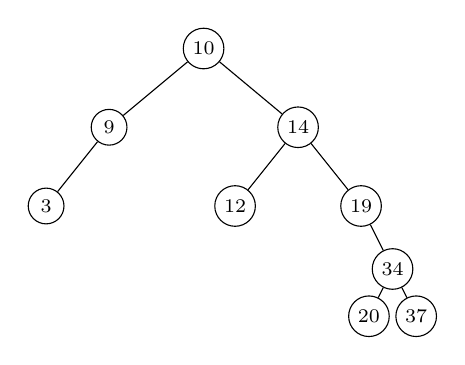
\begin{tikzpicture}[%level distance=5mm,
        level 1/.style={level distance=10mm,sibling distance=24mm},
        level 2/.style={level distance=10mm,sibling distance=16mm},
        level 3/.style={level distance=8mm,sibling distance=8mm},
        level 4/.style={level distance=6mm,sibling distance=6mm},
        font=\scriptsize,inner sep=2pt,every node/.style={draw,circle,minimum size=3ex}]

    \node {10}
    child   {node {9}
            child   {node {3}}
            child [missing]}
    child   {node {14}
            child   {node {12}}
            child   {node {19}
                    child [missing]
                    child   {node {34}
                            child {node {20}}
                            child   {node {37}}}}};
\end{tikzpicture}
\\
2. Left rotation: \\\\
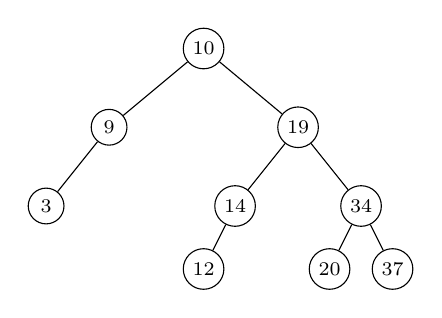
\begin{tikzpicture}[%level distance=5mm,
        level 1/.style={level distance=10mm,sibling distance=24mm},
        level 2/.style={level distance=10mm,sibling distance=16mm},
        level 3/.style={level distance=8mm,sibling distance=8mm},
        level 4/.style={level distance=6mm,sibling distance=6mm},
        font=\scriptsize,inner sep=2pt,every node/.style={draw,circle,minimum size=3ex}]

    \node {10}
    child   {node {9}
            child   {node {3}}
            child [missing]}
    child   {node {19}
            child  {node {14}
                child   {node {12}}
                child   [missing]}
            child   {node {34}
                    child {node {20}}
                    child   {node {37}}}};
\end{tikzpicture}






% \paragraph{Step 3: Insert 12 \\}
% \begin{tikzpicture}[%level distance=5mm,
%         level 1/.style={level distance=10mm,sibling distance=24mm},
%         level 2/.style={level distance=10mm,sibling distance=16mm},
%         level 3/.style={level distance=10mm,sibling distance=16mm},
%         font=\scriptsize,inner sep=2pt,every node/.style={draw,circle,minimum size=3ex}]

%     \node {9}
%     child [missing] % left child
%     child   {node {10} % right child
%             child [missing] % level 2
%             child   {node {12}}};
% \end{tikzpicture}

% \paragraph{Step 4: Insert 14 \\}
% \begin{tikzpicture}[%level distance=5mm,
%         level 1/.style={level distance=10mm,sibling distance=24mm},
%         level 2/.style={level distance=10mm,sibling distance=16mm},
%         level 3/.style={level distance=10mm,sibling distance=16mm},
%         font=\scriptsize,inner sep=2pt,every node/.style={draw,circle,minimum size=3ex}]

%     \node {9}
%     child [missing] % left child
%     child   {node {10} % right child
%             child [missing] % level 2
%             child   {node {12} % level 2
%                     child [missing] % level 3
%                     child   {node {14}}}};
% \end{tikzpicture}

% \paragraph{Step 5: Insert 3 \\}
% \begin{tikzpicture}[%level distance=5mm,
%         level 1/.style={level distance=10mm,sibling distance=24mm},
%         level 2/.style={level distance=10mm,sibling distance=16mm},
%         level 3/.style={level distance=10mm,sibling distance=12mm},
%         font=\scriptsize,inner sep=2pt,every node/.style={draw,circle,minimum size=3ex}]

%     \node {9}
%     child   {node {3} % left child
%         }
%     child   {node {10} % right child
%             child [missing] % level 2
%             child   {node {12} % level 2
%                     child [missing] % level 3
%                     child   {node {14}}}};
% \end{tikzpicture}

% \paragraph{Step 6: Insert 34 \\}
% \begin{tikzpicture}[%level distance=5mm,
%         level 1/.style={level distance=10mm,sibling distance=24mm},
%         level 2/.style={level distance=10mm,sibling distance=16mm},
%         level 3/.style={level distance=10mm,sibling distance=12mm},
%         level 4/.style={level distance=10mm,sibling distance=8mm},
%         font=\scriptsize,inner sep=2pt,every node/.style={draw,circle,minimum size=3ex}]

%     \node {9}
%     child   {node {3} % left child
%         }
%     child   {node {10} % right child
%             child [missing] % level 2
%             child   {node {12} % level 2
%                     child [missing] % level 3
%                     child   {node {14} % level 3
%                             child [missing] % level 4
%                             child   {node {34}}}}};
% \end{tikzpicture}

% \paragraph{Step 7: Insert 19 \\}
% \begin{tikzpicture}[%level distance=5mm,
%         level 1/.style={level distance=10mm,sibling distance=24mm},
%         level 2/.style={level distance=10mm,sibling distance=16mm},
%         level 3/.style={level distance=10mm,sibling distance=12mm},
%         level 4/.style={level distance=10mm,sibling distance=8mm},
%         level 5/.style={level distance=8mm,sibling distance=6mm},
%         font=\scriptsize,inner sep=2pt,every node/.style={draw,circle,minimum size=3ex}]

%     \node {9}
%     child   {node {3} % left child
%         }
%     child   {node {10} % right child
%             child [missing] % level 2
%             child   {node {12} % level 2
%                     child [missing] % level 3
%                     child   {node {14} % level 3
%                             child [missing] % level 4
%                             child   {node {34} % level 4
%                                     child   {node {19}} % level 5
%                                     child   [missing]}}}};
% \end{tikzpicture}

% \paragraph{Step 8: Insert 37 \\}
% \begin{tikzpicture}[%level distance=5mm,
%         level 1/.style={level distance=10mm,sibling distance=24mm},
%         level 2/.style={level distance=10mm,sibling distance=16mm},
%         level 3/.style={level distance=10mm,sibling distance=12mm},
%         level 4/.style={level distance=10mm,sibling distance=8mm},
%         level 5/.style={level distance=8mm,sibling distance=6mm},
%         font=\scriptsize,inner sep=2pt,every node/.style={draw,circle,minimum size=3ex}]

%     \node {9}
%     child   {node {3} % left child
%         }
%     child   {node {10} % right child
%             child [missing] % level 2
%             child   {node {12} % level 2
%                     child [missing] % level 3
%                     child   {node {14} % level 3
%                             child [missing] % level 4
%                             child   {node {34} % level 4
%                                     child   {node {19}} % level 5
%                                     child   {node {37}}}}}};
% \end{tikzpicture}

% \paragraph{Step 9: Insert 20 \\}
% \begin{tikzpicture}[%level distance=5mm,
%         level 1/.style={level distance=10mm,sibling distance=24mm},
%         level 2/.style={level distance=10mm,sibling distance=16mm},
%         level 3/.style={level distance=10mm,sibling distance=12mm},
%         level 4/.style={level distance=10mm,sibling distance=8mm},
%         level 5/.style={level distance=8mm,sibling distance=6mm},
%         level 6/.style={level distance=8mm,sibling distance=6mm},
%         font=\scriptsize,inner sep=2pt,every node/.style={draw,circle,minimum size=3ex}]

%     \node {9}
%     child   {node {3} % left child
%         }
%     child   {node {10} % right child
%             child [missing] % level 2
%             child   {node {12} % level 2
%                     child [missing] % level 3
%                     child   {node {14} % level 3
%                             child [missing] % level 4
%                             child   {node {34} % level 4
%                                     child   {node {19} % level 5
%                                             child [missing] % level 6
%                                             child  {node {20}}} % level 6
%                                     child   {node {37}}}}}};
% \end{tikzpicture}

$$ \blacksquare $$

\newpage

% Q2-b-1
\section*{Q2-b-1}

\text{Q: }
\paragraph{On the tree shown below, show each step of deleting the keys p, d, h. \\}
\text{\newline}
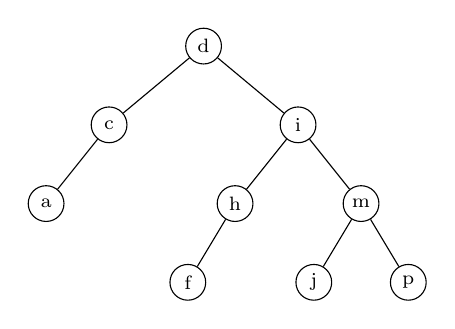
\begin{tikzpicture}[
        level 1/.style={level distance=10mm,sibling distance=24mm},
        level 2/.style={level distance=10mm,sibling distance=16mm},
        level 3/.style={level distance=10mm,sibling distance=12mm},
        level 4/.style={level distance=10mm,sibling distance=8mm},
        font=\scriptsize,inner sep=2pt,every node/.style={draw,circle,minimum size=3ex}]

    \node{d}
    child   {
            node{c}
            child   {node{a}}
            child   [missing]
        }
    child   {
            node{i}
            child   {
                    node{h}
                    child   {node{f}}
                    child   [missing]
                }
            child{
                    node{m}
                    child   {node{j}}
                    child   {node{p}}
                }
        };

\end{tikzpicture}

\paragraph*{Step 1: Delete p \\}
\text{Hold on, Latex is not a good fit for this question.}
\newline
\text{I will leave some space here for the hand-drawn tree.}
\vfill{$$\blacksquare$$}
\newpage

% Q2-b-2
\section*{Q2-b-2}
\text{Q: }
\paragraph*{On the tree shown below, show each step of deleting the keys p, d, h. \\}
\text{\newline}
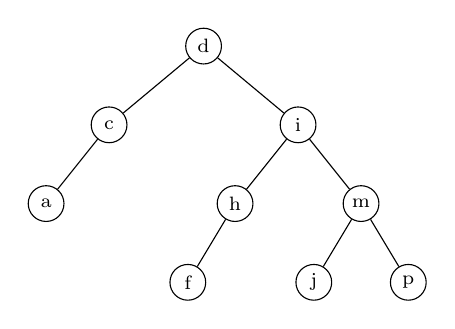
\begin{tikzpicture}[
        level 1/.style={level distance=10mm,sibling distance=24mm},
        level 2/.style={level distance=10mm,sibling distance=16mm},
        level 3/.style={level distance=10mm,sibling distance=12mm},
        level 4/.style={level distance=10mm,sibling distance=8mm},
        font=\scriptsize,inner sep=2pt,every node/.style={draw,circle,minimum size=3ex}]

    \node{d}
    child   {
            node{c}
            child   {node{a}}
            child   [missing]
        }
    child   {
            node{i}
            child   {
                    node{h}
                    child   {node{f}}
                    child   [missing]
                }
            child{
                    node{m}
                    child   {node{j}}
                    child   {node{p}}
                }
        };

\end{tikzpicture}

\paragraph*{Step 2: Delete d \\}
\text{Hold on, Latex is not a good fit for this question.}
\newline
\text{I will leave some space here for the hand-drawn tree.}

\vfill{$$\blacksquare$$}
\newpage

% Q2-b-3
\section*{Q2-b-3}
\text{Q: }
\paragraph*{On the tree shown below, show each step of deleting the keys p, d, h. \\}
\text{\newline}
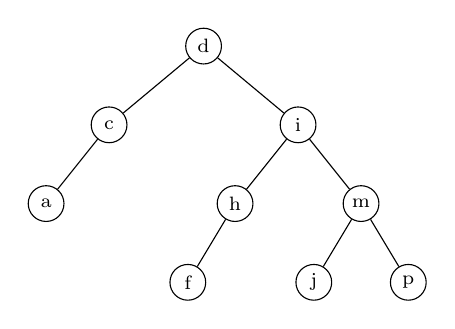
\begin{tikzpicture}[
        level 1/.style={level distance=10mm,sibling distance=24mm},
        level 2/.style={level distance=10mm,sibling distance=16mm},
        level 3/.style={level distance=10mm,sibling distance=12mm},
        level 4/.style={level distance=10mm,sibling distance=8mm},
        font=\scriptsize,inner sep=2pt,every node/.style={draw,circle,minimum size=3ex}]

    \node{d}
    child   {
            node{c}
            child   {node{a}}
            child   [missing]
        }
    child   {
            node{i}
            child   {
                    node{h}
                    child   {node{f}}
                    child   [missing]
                }
            child{
                    node{m}
                    child   {node{j}}
                    child   {node{p}}
                }
        };

\end{tikzpicture}

\paragraph*{Step 3: Delete h \\}
\text{Hold on, Latex is not a good fit for this question.}
\newline
\text{I will leave some space here for the hand-drawn tree.}
\vfill{$$\blacksquare$$}
\newpage

% Q2-c
\section*{Q2-c}
\text{Q: }
\paragraph*{Carefully consider the tree below. \\}
\text{\newline}
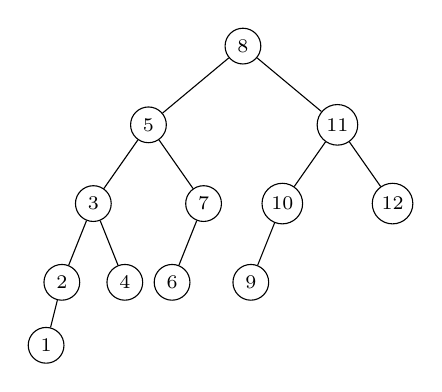
\begin{tikzpicture}[
        level 1/.style={level distance=10mm,sibling distance=24mm},
        level 2/.style={level distance=10mm,sibling distance=14 mm},
        level 3/.style={level distance=10mm,sibling distance=8mm},
        level 4/.style={level distance=8mm,sibling distance=4mm},
        font=\scriptsize,inner sep=2pt,every node/.style={draw,circle,minimum size=3ex}]

    \node{8}
    child   {
            node{5}
            child   {
                    node{3}
                    child   {node{2}
                            child {node{1}}
                            child [missing]
                        }
                    child   {node{4}}
                }
            child   {node{7}
                    child   {node{6}}
                    child   [missing]
                }
        }
    child   {
            node{11}
            child   {
                    node{10}
                    child   {node{9}}
                    child   [missing]
                }
            child{node{12}}
        };
\end{tikzpicture}

\begin{itemize}
    \item [-] If we start with an empty AVL tree, what sequence of insertions would result in this tree?
    \item [-] Show each step of deleting key 11.
\end{itemize}

\text{As usual, I will leave some space here for the hand-drawn tree.}
\vfill{$$\blacksquare$$}
\newpage

% Q4
\section*{Q4}
\text{Q: }
\text{Consider an ADT consisting of a set S of distinct integers and the following operations: \\}

\begin{itemize}
    \item search(S, x): Return true if x is in S and false otherwise.
    \item insert(S, x): Insert the element x into the set S.
          This operation has no effect if x is already in S.
    \item \text{delete(S, x): Delete the element x from the set S. This operation has no effect if x is not in S.}
    \item min difference(S): Given a set S with size of at least 2, return a pair of distinct integers (x, y),
          \newline
          with x $\in$ S, y $\in$ S, with the minimum absolute difference, i.e.
          \newline
          $\forall x', \forall y', (x' \neq y' \rightarrow |x - y| \leq |x' - y'|)$
\end{itemize}
\paragraph{}
Your task is to design a data structure to implement this ADT, \\
such that all operations are performed in $\mathcal{O} (\log\ n)$ time, \\
where $n = |S|$. You will do so by augmenting our familiar AVL tree.

\begin{enumerate}
    \item Describe all information that will be stored in the nodes.
    \item Provide pseudo-code for each required operation.
    \item Justify why your algorithms are correct and why they achieve the required time bound.
\end{enumerate}

\newpage
\mbox{}
\vfill{$$\blacksquare$$}
\end{document}